\chapter{Design of the Experiments}

\section{Concepts and Variables}

The overall plan of this work was to measure the rates of germination for a wide
range of species and for a wide range of conditions. Plots or graphs were constructed
with the number of seeds (or the percentage) on the vertical axis and time on the
horizontal axis. These are rate plots, and they are the most sensitive way of detecting
the effects of any treatments and conditioning of the seeds. It is emphasized that these
rate plots can be used without any recourse to mathematical analysis. They can be
treated as empirical plots and used simply as a: delicate sensor to detect internal
changes in the seeds that were caused by any prior treatments.

Work on seed germination in the past has been directed towards growing
plants. The present work has a different philosophy. Seed germination is a science in
itself and a fascinating one replete with a multitude of phenomena. An. understanding
of this science will best serve the goal of growing plants from seeds.
All seed bearing plants must have a delay mechanism as stated in Chapter 1.
The 5\% that use physical mechanisms are treated in Chapter 9. A question arises as
to the nature of the chemical mechanisms used by the other 95\%. The word chemical
is used here in its broadest sense. It includes destruction of a specific chemical
inhibitor, conformational changes in proteins to go from enzymatically active to inactive
forms, restructuring of membranes to change their permeability, and possibly the
formation of promoters.

\textbf{Temperature} is a major variable in seed germination. Virtually all of
the experiments were conducted at either 40 or 70 deg. F. These two
temperatures were chosen first for convenience. The temperature of 70 is the
temperature at which most rooms are kept, and 40 is the temperature at which
refrigerators are generally set.  These two temperatures also roughly
correspond to the temperatures of the winter and summer seasons. Also there has
been much work done on the chilling periods required by fruit trees in order to
prepare the buds for opening and growth in spring. It had been lound,that
temperatures in the range 35-40 were most effective, and temperatures below
freezing were ineffective.

As the work progressed it was found over and over that destruction of delay
mechanisms would take place at either 40 or 70 but not both. This means that these
processes undergo an enormous change in rate somewhere between 40 and 70. It is
likely that nature has evolved these chemical processes to take place in just two
temperature regions so that the plant has a well defined winter metabolism and a well
defined summer metabolism. It is likely that 40 and 70 are near the center of these two
temperature regions. It is proposed that temperature variations of the order of five to
ten degrees centered around 40 or 70 have small effects on rates, but the jump from
the region around 40 to the region around 70 causes enormous changes in rates.
Much more work will be needed to firmly establish this principle.

Germinations also tend to take place either in the 40 region or the 70 region of
temperatures. However, with germinations the division is not so complete. Examples
were found where germination would take place at both 40 and 70.

There have been reports that temperatures in the 90-100 region are required for
the germination of certain species and that short exposures of temperatures as high as
180 initiate germination (see Gomphrena, Kalmia, and Mimosa in Chapter 20). In the
present work Gomphrena haageana and Mimosa pudica were the only species in
which temperatures other than 40 or 70 were investigated. The generally successful
germination of nearly 2500 species at 40 or 70 indicates that temperatures other than
40 and 70 are rarely needed.

\textbf{Time} is another critical variable. Nearly all the work was conducted using
periods of three months at one temperature followed by a shift to the other
temperature. This led to a series of alternating cycles each of three months duration.
The three month period was chosen because it corresponds roughly to the length of
the winter and summer seasons and because studies on fruit trees had shown that
three months of chilling was about the amount required.

By using rate studies and rate techniques it was quite easy to show that the
three month periodswere a good choice. For example, Eranthis hyemalis has a delay
mechanism that is destroyed at 70. Samples were held at 70 and portions periodically
removed and shifted to 40 where germination took place. It was possible from rate
plots of the germination at 40 to construct the rate plot for the destruction of the
inhibitor system at 70 and to show that destruction of the inhibitor system was
complete at the end of three months at 70.

Occasionally the rate plots showed that times longer than three months were
needed. When this was the situation, longer times were investigated. Sometimes the
rate plots showed that times shorter than three months could have been used.

\textbf{Dry storage} is a critical variable. All seeds are ultimately killed if dry storage
is continued long enough (Chapter 13). The rates of dieing in dry storage vary widely
and are a taxonomic character for each species. Some species cannot tolerate even a
week or two of dry storage and others retain viability in dry storage for over a hundred
years. These death rates follow a rate curve. There is no point where all the seeds
suddenly die. These death rates depend on temperature and relative humidity, and
even the best literature studies did not control these variables very well. There is
some anecdotal evidence to indicate that seeds that have been stored too long and
are near death will germinate, but the seedlings are weak and may not survive.

Some seeds \textit{require} a period of dry storage to destroy inhibitors, and these are
termed D-70 germinators (Chapter 5). The rates of the destruction processes vary
widely and are a taxonomic character for each species. With these D-70 germinators
there are opposing processes in dry storage. One is destroying inhibitors and favoring
germination and the other is the dieing in dry storage which is unfavorable to
germination. There will be an optimum time or range of times for the dry storage.
When fresh seeds were obtained, they were subjected to various treatments
both in the fresh state and after dry storage. Six months was the usual time for the dry
storage, but a few experiments were conducted for longer and shorter times where the
data indicated that studies on other times would be of value.

Early in the work the seeds were subjected to dry storage at both 40 and 70. A
number of experiments showed that there was little difference in viability between
seeds dry stored at 40 relative to seeds dry stored at 70. Asa result dry storage at 40
was abandoned, and all later experiments used only dry storage at 70. Where a
difference occurred as in Hyacinthus orientalis, death rates at 40 were slower than at
70, but not by enough to be a solution to the problem of storing the seeds. This
problem is discussed in more detail in Chapter 13.

Most of the samples of seeds were received in midwinter and had already been
subjected to some dry storage at unknown temperatures and relative humidities. This
introduced some uncertainty into the data in Chapter 20 and is a potential cause of
results that appear to be inconsistent.

\textbf{Light} is an important variable (Chapter 11), and one that has often been poorly
controlled in past work. Light stimulated the germination in many species. Where it
stimulated germination, it was often an absolute requirement. This is contrary to past
literature which generally regarded light as "favoring, not favoring, or having no effect"
on germination.

In the present work only one light intensity was used and only one timing cycle
(twelve hours on twelve hours off). A vast number of experiments could be constructed
varying light intensity and timing cycles. It is expected that the results will not lead to
improved germination procedures, but this will have to be tested.

\textbf{Oscillating temperatures} were required for germination by some species,
and this behavior was totally unexpected (Chapters 10 and 19). It was found that
some species would germinate under outdoor conditions, but not under the alternating
three month cycles at 40 and 70. There are two explanations for this. One is that
these are the first examples of chemical processes that proceed only under conditions
of oscillating temperatures. Such an effect is theoretically possible, but has not been
found to the best of my knowledge in small molecule chemistry. Experiments on
germination of Cleome.(Chapter 10) indicate that this is the correct explanation, but
more work is needed The other explanation is that germination is occurring at some
temperature between 40 and 70 and not at 40 or 70: This is regarded as less likely,
but the definitive experiments of conducting germination at 40, 50, 60, and 70 have not
yet been done.

\textbf{Gibberelins} are a critical variable. Because of two recent papers (refs. 9 and
10, see Chapter 12) treatment with and without gibberelic acid-3 (GA-3) has become a
standard treatment given to every sample of seeds. It is important to control this
variable. It has been a cause of inconsistent results.

\textbf{Disinfection of Seeds} was not used in the present work. There was much
evidence that pathogenic fungi were not a problem and that only dead seed and
empty seed coats were attacked by fungi in the moist paper towels. First was the
observations that fungal spots were generally few and isolated. Close examination
with a lens showed that these were associated with empty seed coats or pieces of
chaff and debris. Early evidence of fungal attack is sticking of the seed coat to the
towel, appearance of a tiny droplet of white fluid at the apex of the seed, softness of the
seed, and ultimately the fungus itself surrounding the seed coat. Such fungal spots
and rotting seeds were removed by forceps or a toothpick. If they became too
numerous, the unrolled seed was moved to a fresh towel. The remaining seeds
stayed firm and in many cases germinated months later and sometimes years later,
evidence that the fungi were not pathogenic and were not attacking live seed.

The second line of evidence was that the fungal attacks were spaced. They did
not expand in concentric rings of growth nor did they progress along any front. Both
would have happened if the fungi had been pathogenic. Third was the behavior of
some species in Berberidaceae and flanunculaceae. Certain of these do not survive
dry storage although the seed shows no outward sign of having died. When such
seed that has been dry stored for six months is placed in a moist towel, it is completely
rotted in a week or two. In contrast fresh seed of the same species stayed firm and
unrotted in the moist towels for months and even over a year until they finally
germinated, and throughout this time there was no evidence of fungal attack. Fourth
was the behavior of a few species, Lindera benzoin and Skimmia japonica for
example, where about half the seed rotted within a week or two after encountering
moisture while the rest of the seed ultimately germinated and produced vigorous
seedlings. The seeds that rotted must have been internally infected for such rapid
fungal attack.

Finally John Gyer has tried a number of methods for external disinfection of a
strain of lima bean that he and his wife Janet market. None were effective and many
were deleterious. Spraying the vines with fungicides at the time of blooming seemed
to have some effect in lowering the percentage of internally infected seeds.
Several factors were found to have little importance despite reports in past
literature. Soaking seeds in water has often been recommended. Of course seeds in
fruits usually need to have the inhibitors removed by washing (Chapter 9), but that is
something different than proposing that soaking alone is favorable. Table 8-1 in
Chapter 8 gives some data comparing soaking for one week relative to soaking for
four weeks. In general there was no advantage in the longer periods of soaking. It is
concluded that the supposed favorable effects of soaking are largely a myth.

Removal of seed coats has been claimed to be beneficial for germination (ref.
11) because the seed coats were thought to be repositories for germination inhibitors.
Not only is this unlikely from a chemical viewpoint but no evidence of this could be
found in the present work. From the chemical viewpoint the outer seed coat (the
pericarp) and the inner seed coat (the testa) are lignaceous, insoluble, high polymers
that are not suited to be repositories for water soluble or oil soluble germination
inhibitors. From the experimental viewpoint a number of experiments were conducted
on species of Acer, Corylus, Prinsepia, and Quercus. No evidence was found for seed
coats as a repository for germination inhibitors and The claims for Acer sacharum and
Corylus avellana were specifically tested. It is important to differentiate the claims of
inhibitors in seed coats from the problem of an impervious seed coat. The latter can
be readily detected by simply making a hole in the seed coat instead of total removal
of the seed coat.

A minor problem involved empty seed coats. It is characteristic of some species
to produce quantities of empty seed coats or produce empty seed coats some years
and viable seeds other years. Some samples of seeds were found to contain up to
100\% empty seed coats which cannot be detected by the outward appearance.
Species of spruce, the beech nut, and Adonis vernalis are particularly prone to this
behavior. It is proposed that this may have survival value. Seeds are eaten by many
animals and insects. Suppose something eats the seeds, if it opens many seed coats
only to find them empty, it will become discouraged and diminish efforts to eat the
seeds. This survival techique is well known in certain fish such as grunions which
spawn in great numbers in a highly localized area in a single night of the year.

\section{Experimental Procedures}

\textbf{Basic Procedure.} The only materials needed for the basic procedure are (A)
ScotTowels, a high wet strength paper towel made by the Scott Paper Company; (B)
Baggies. a polyethylene bag made by the Mobil Chemical Company; and (C) Pilot
extra fine point permanent markers made by the Pilot Corporation of America. A
perforated section of paper towel is torn off and folded in half three times in alternating
directions to give a rectangular pad 2.5 x 4.5 inches. The name of the species and any
other information is written on the outside of the pad with the Pilot marker. The final
(third) fold is opened, and the towel is moistened with water. The seeds are sprinkled
on the moist open pad. The third fold is closed and the whole placed in a Baggie.
Fold the Baggie several times so that evaporation of water from the towel is inhibited,
yet leaving ample access to air to insure aerobic conditions. The drawings (\ref{fig:towel})
illustrate this procedure.

\begin{figure}[hbt!]

\begin{subfigure}{.20\linewidth}
  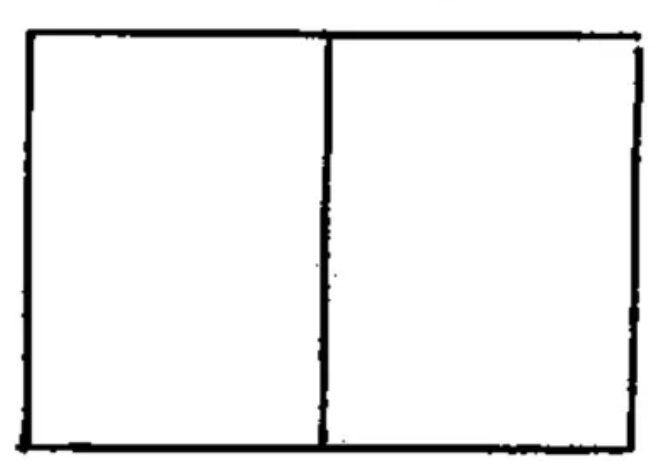
\includegraphics[width=\linewidth]{figs/towel1.png}
  \caption{Moisten the folded towl}
  % \label{x}
\end{subfigure} % \hfill % <-- "\hfill"
\hfill
\begin{subfigure}{.20\linewidth}
  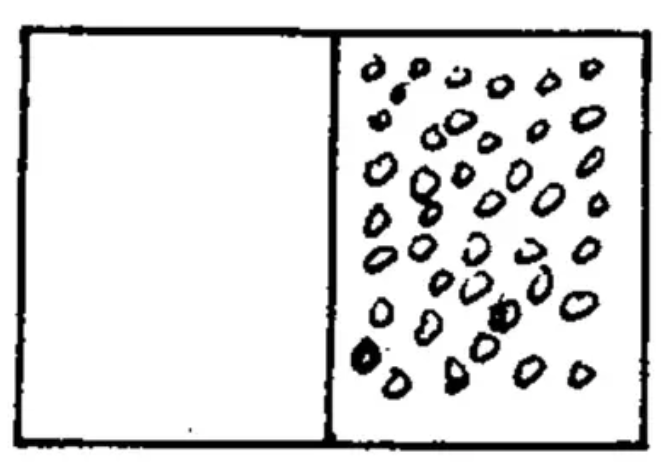
\includegraphics[width=\linewidth]{figs/towel2.png}
  \caption{Sprinkle the seeds on one side}
\end{subfigure}
\hfill
\begin{subfigure}{.20\linewidth}
  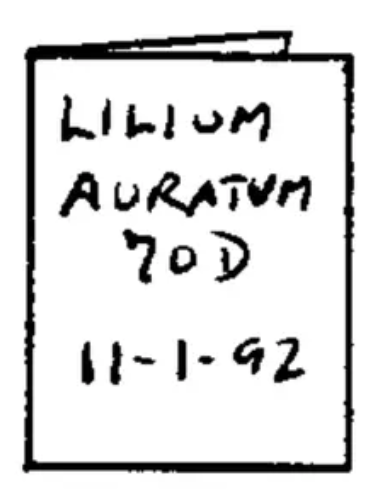
\includegraphics[width=.75\linewidth]{figs/towel3.png}
  \caption{Fold the towel}
  % \label{velcomp}
\end{subfigure}
\hfill
\begin{subfigure}{.20\linewidth}
  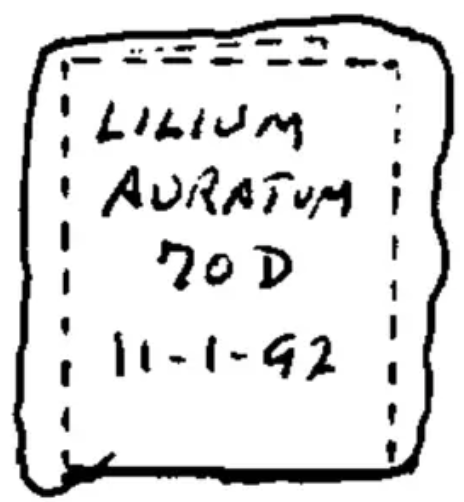
\includegraphics[width=.75\linewidth]{figs/towel4.png}
  \caption{Place in Baggie, fold loosely}
  % \label{estcomp}
\end{subfigure}

\caption{Towel Procedure}
\label{fig:towel}

\end{figure}


A special warning is made about certain brands of paper towels that are
advertised for their softness. These become mushy very quickly. It is important to use
high wet strength paper towels, and the plain white type are preferred. Also a special
warning against Ziploc bags and other polyethylene bags that are of thicker
polyethylene film and are constructed to seal tightly. Polyethylene film is permeable to
oxygen but not water (even though water is the smaller molecule) so that by using the
thinner polyethylene, the permeablility of the film to oxygen helps maintain aerobic
conditions.

The paper towels remain moist for periods of months and only need to be
remoistened at periods of two months or longer. The towels are inspected and the
germinated seeds counted at least once every seven days and as often as each day if
germination is occurring at a rapid rate. If there is debris or other material that starts to
rot, the seeds are transferred to new moist towel. Dead seeds rot in month or two
and are removed. It was usually necessary to transfer ungerminated seeds to a new
towel about every three months as even the ScotTowels ultimately disintegrate. The
edge of a dull knife blade was a particularly convenient instrument for transferring
seeds from one towel to another. Samples of seeds were started at both 40 and 70
and shifted to the alternate temperature every three months.

This method of germinating seeds in moist paper towels was first described in a
talk given by Margery Edgren at an annual meeting of the American Rock Garden
Society, and I am much indebted to the inspiration of this talk. The procedure can be
used to germinate seeds for growing on to plants as described in Chapter 14. It is a
highly efficient procedure for seeds that have extended germinations since watering is
minimal and little space is required. About twenty pads can be stacked in each
Baggie, and about five hundred experiments can be conducted in one cubic foot. I
dread to think of earlier investigators with rows and rows of pots or Petri dishes that
needed almost daily attention.

There was the possibility that chemicals used in processing the paper towels
had an effect on germination. The fact that highly successful germination was
achieved in all but perhaps five or less species out of the nearly 2500 examined
indicates that this was not a factor.

\textbf{Photoexperiments.} The photoexperiments were started in the same way as
the basic procedure except that the seeds were placed on top of the 2.5 x 4.5 inch pad
of moist paper towel. Each moist pad was placed in its own Baggie, and the Baggie
was folded several times as in the basic procedure. -These were placed at a distance
of eight inches under two fluorescent lights. These lights were daylight type, four foot
long, and forty watts each. The lights were timed to provide alternating twelve hours of
light and twelve hours of dark. The effects of light were sometimes complex and
changed by prior treatment as discussed in Chapter 11.

Outdoor Treatment. The outdoor conditions simply consisted of placing the
polyethylene bags containing the towels and seeds outdoors in a shed. The only
important precaution is to prevent any direct sunlight from striking the polyethylene
bags as that would lead to overheating.

\textbf{Gibberelic Acid-3 (GA-3).} The GA-3 experiments started with the same
basic procedure. After opening the third fold and moistening the towel, two inserts
were made before sowing the seeds. The first was a 3 x 3 inch piece of polyethylene
cut from a Baggie. The second was a small piece (2.5 x 2.5 inches) of ScotTowel
folded three times to give a rectangular pad 0.5 x 1.0 inches. This is moistened and
placed on top of the polyethylene. The seeds are placed on top of this inner pad and
one cubic millimeter of 95\% GA-3 is sprinkled on top of the seeds. This amount of GA-3
is about the amount that can be balanced on the 0.5 mm tip of a toothpick using a
type of toothpick that is pointed at both ends. The whole is folded once and placed
inside a Baggie as in the basic procedure. These steps are illustrated by \ref{fig:towel-ga3}.

\begin{figure}[hbt!]

\begin{subfigure}{.20\linewidth}
  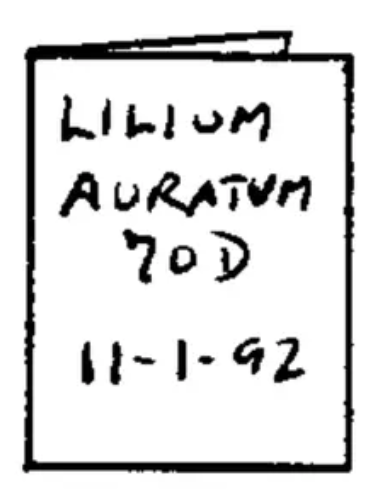
\includegraphics[width=\linewidth]{figs/towel3.png}
  \caption{Towel folded}
  % \label{x}
\end{subfigure} % \hfill % <-- "\hfill"
\hfill
\begin{subfigure}{.20\linewidth}
  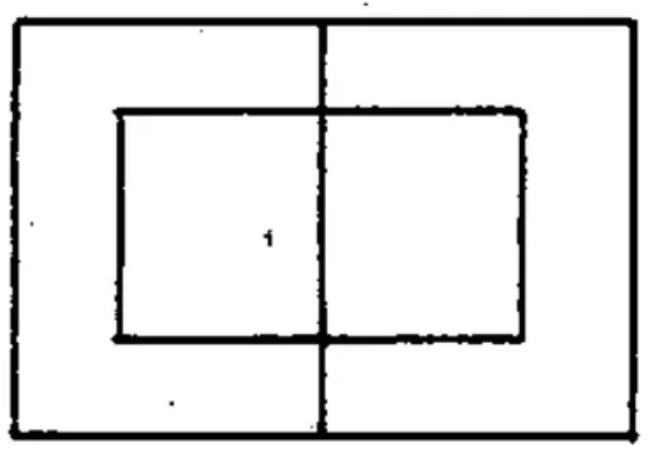
\includegraphics[width=\linewidth]{figs/towel-pi.png}
  \caption{Towel with polyethylene insert}
\end{subfigure}
\hfill
\begin{subfigure}{.20\linewidth}
  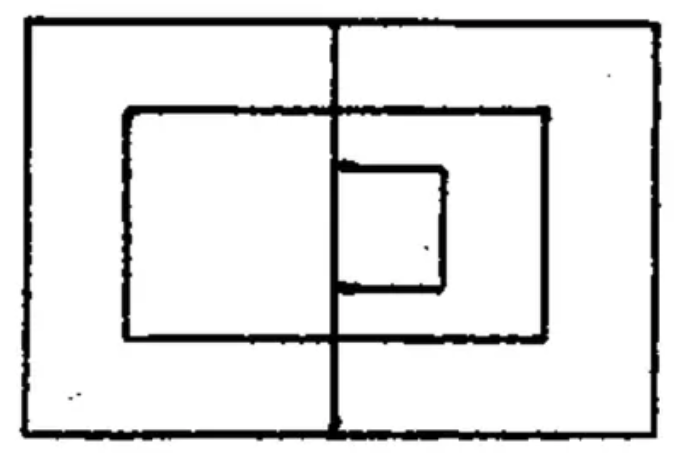
\includegraphics[width=.75\linewidth]{figs/towel-pi2.png}
  \caption{Inner pad inserted, moistened, and ready for seed}
  % \label{velcomp}
\end{subfigure}
\hfill
\begin{subfigure}{.20\linewidth}
  Sow seed, add GA-3, fold, insert in Baggie, and loosely fold as before
\end{subfigure}

\caption{Towel with GA-3}
\label{fig:towel-ga3}

\end{figure}



It was important to adopt reasonably hygienic techniques since some species
such as Evodia danielli were very sensitive to GA-3, and it would not do to
contaminate the work area with GA-3. Everything used to handle the GA-3 was
washed after use.

The beauty of the above procedure is that it does not require any weighing,
volume measurements, or filtering. The experiments take up very little space, and they
can be set up rapidly and examined rapidly. The size of the inner pad is such that it
takes about six drops of water to moisten it and with the one cubic millimeter of GA-3
this works out to be a concentration of about 1000 ppm, the concentrations found to be
about optimum in other work (refs. 9 and 10). By applying the GA-3 to only the inner
pad, the GA-3 is used most efficiently. The moist outer pad serves as a water reservoir
maintaing 100\% relative humidity so that the small inner pad does not dry out. The
amount of GA-3 can be reduced or increased and the time of exposure varied by
simply transferring the seeds from the GA-3 experiment to a fresh moist paper towel. A
further advantage is that there are no solutions of GA-3 that have to be discarded.
Note that reuse of GA-3 solution would lead to uncertainties because of varying
absorption of GA-3 by seed coats as well as the seeds.

A further beauty of the above procedure is that it can be used b y every home
gardener, and it can be used for the growing of plants. As soon as a seed germinates,
it is removed and planted as described in Chapter 14. If there are problems with the
seedlings being weakened by etiolation, the dosages and times of contact can be
adjusted as described in Chapter 12.

\textbf{Washing Seeds in Fruits and Berries.} Seeds in fruits and berries
generally contain germination inhibitors in the pulp and these seeds were \textit{always}
washed and cleaned. The abbreviation WC is used to indicate that the seeds were
washed and cleaned. Some fruits such as those of Euonymus contain inhibitors that
are oil soluble rather than the usual water soluble, and such seeds must be washed
with detergents. This subject is covered in Chapter 8. Generally seeds in fruits have a
channel through the seed coat so that impervious seed coats are virtually never found
although Prinsepia is an exception. Thus germination is not benefitted by physical
treatments of the seed coat. Fruits of a number of Ericaceae such as Vaccinium use
another delay mechanism so that washing is more for convenience than necessity.
Impervious Seed Coats. Certain species use the mechanism of an
impervious seed coat to prevent germination before dispersal of the seed (Chapter 9).
Many treatments have been recommended for such seed, but the \textit{only treatment} that
gives reliable and reproducible (and usually dramatic) effects is to physically produce
a hole in the seed coat.

Such holes in the seed coats were made in several ways. Large seeds could
be rubbed against a file or sandpaper until the endosperm showed. It is advisable to
make this hole away from the embryo to avoid physical injury. With bean shaped
seeds of Fabaceae, this means making the hole on the convex edge of the seed.
Every attempt was made to use this reliable method of making a hole. However, there
were some seeds that were so small that recourse was made to rubbing them between
sandpaper.

Soaking in sulfuric acid has often been recommended for seeds with
impervious seed coats, but I advise against it. First of all the temperatures,
concentrations of sulfuric acid, and times of exposure all have to be worked out for
each separate species. More important sulfuric acid is dangerous to use. Many years
ago there were tragic accidents involving loss of eyesight using sulfuric acid, and this
is one of the principal reasons for requiring safety goggles in all chemistry
laboratories. This is no trivial caution from someone outside the field as I was
internationally known for my work and publications on rates and equilibria in sulfuric
acid.

\section{Results that Appear to be Inconsistent}

There will be the temptation for readers to cite some anecdote that appears to
be inconsistent with the results herein, and the experiments themselves occasionally
gave the appearance of being inconsistent. Five factors were identified that could lead
to such apparent inconsistencies.

Seeds are stored under a variety of conditions. To cite an extreme example,
seeds could be stored in a sealed polyethylene bag. Since polyethylene films do not
transmit water, seeds stored in this way are in effect being stored under conditions of
100\% relative humidity or close to it. Such seed is in effect being stored moist and the
behavior will be that of seeds stored moist not dry.

The dieing of seeds in dry storage is a chemical rate process. It is like
radioactive decomposition. A certain amount dies in each time period. Even after
extended dry storage there may remain a few viable seeds.

A most serious problem is the presence or absence of gibberelin producing
fungi in the medium in which the seeds are planted. Since gibberelins such as GA-3
can have a dramatic effect on germination, this factor must be rigidly controlled to get
consistent results. Fortunately in the present work aseptic conditions were used and
the factor was controlled. Much of the past work reported in the literature used soils
and composts and this factor was not controlled. The uncertainties caused by this
factor places much of the past work under a cloud of uncertaintly. An interesting
anecdotal example involves the rosulate violas of the Andes. English collectors had
brought back seeds of these, but germinations were only rarely observed, and such
germinations could not be correlated with any particular treatment. The presence or
absence of gibberelins was probably the unknown factor.

A minor problem relates to variations in the seeds produced. Rarely species
produce two kinds of seed with different behaviors. There have also been reports that
seeds of a particular species differed when produced from different geographical
areas or from years with different weather patterns. This problem was not actively
investigated, but there were many times that two or more samples of seeds of a
species were obtained from widely different areas and sources. Generally the same
pattern of germination was observed, so I am inclined not to attach much importance to
this factor as a cause of apparent inconsistencies.

The fifth factor is the problem of defining a species. Different strains of a
species could have different germination behavior. In the limit two strains could be
identical in all respects except the nature of their seed germination.
The results herein show that many seeds can be stored for six months or more
in a moist state by careful choice of the temperature for storage. For example Eranthis
hyemalis and Fritillaria acmopetala germinate only at 40 deg. F so that the seeds can
be stored moist for many months at 70. Conversely species that germinate at 70 (and
not 40) could be stored for many months in a moist state at 40. For the many seeds
that cannot tolerate dry storage, it is necessary to develop procedures for storing the
seeds in a moist state.

Seeds can be stored moist by placing them in the moist paper towels, placing
the towel in a polyethylene Baggie, and folding loosely. Commercial seed houses are
urged to start storing and distributing seeds of certain species in the moist state.
A question that has not been investigated is whether the moist storage could be
conducted in sealed systems. It may vary from species to species. If it worked, the
seeds could be sealed in polyethylene packets containing a drop of water. Already
some seed houses distribute some of their seeds in sealed packets (Thompson and
Morgan) so that they are already set up for such procedures. Again it is emphasized
that the feasibility of such distributions in the moist state will have to be established for
each species. Note that thin polyethylene films will transmit oxygen. It may well be
that sealed packets will work with polyethylene films but not other plastic films.

